\chapter*{Závěr}
\addcontentsline{toc}{chapter}{Závěr}
V rámci této práce byla dle zadaných požadavků navržena, implementována a otestována webová aplikace pro procházení a vizualizaci dat z grafových databází. To, jak jsou data zobrazena a jakým způsobem je lze procházet popisuje konfigurace.

Uživatel si může do aplikace přidat vrcholy reprezentující existující entity a ty může expandovat a rozšiřovat tak graf o nové vrcholy. Aplikace poskytuje uživateli dodatečné informace o vrcholech, obarvuje je podle jejich typu, umožňuje filtrovat graf a podporuje několik layoutů, jak může být graf zobrazen. Pro snazší práci lze vrcholy seskupovat do skupin, a je možné si vrcholy zobrazit tak, aby je bylo snadné procházet po jejich sousedech.

\section{Možnosti vylepšení}
Tato kapitola rozebírá možné způsoby, jak aplikaci rozšířit do budoucna a možnou implementaci, jak tyto rozšíření provést.

\subsection*{Rozhraní mezi serverem a klientem}
Aktuálně je rozhraní navrženo tak, že serveru lze posílat požadavky samostatně. Toto řešení je nicméně nevyhovující v případě, kdy bude klient vyžadovat odpovědi na více požadavků současně. Budou-li poslány v jedné zprávě, kromě snížení komunikace mezi serverem a klientem bude moci server optimalizovat dotazy na datové zdroje. Kupříkladu dvě expanze lze teoreticky spojit do jednoho SPARQL dotazu.

Server také může posílat data, o která klient nežádal, v případě, že se bude domnívat, že je klient může požadovat. Například když klient požádá o \texttt{view-sets}, může server rovnou poslat \texttt{preview} na výchozí pohled, neboť o něj bude klient zřejmě žádat.

\subsection*{Cachování}
Problém cachování již v této práci rozebírán byl. S každým požadavkem klienta se server dotazuje datových zdrojů. Tato operace je časově náročná a zbytečně dochází k vytěžování datových zdrojů.

Kupříkladu SPARQL endpoint Wikidat má omezení na počet požadavků a při vysoké aktivitě klienta může server dostat IP ban.

Možnosti cachování jsou následující:
\begin{itemize}
    \item Cachovat výsledky jednotlivých dotazů. Například budou cachována data expanze pro každý vrchol kompletně zvlášť. Toto řešení je jednoduché, nicméně náročné na paměť, neboť jednotlivé vrcholy budou uložené několikrát.
    \item Cachovat malé bloky a ty pak sestavovat. V případě s expanzí bude uložen pouze seznam IRI vrcholů a data k vrcholům budou uložená samostatně. Tak dojde k omezení všech redundantních informací. U každého bloku bude uložen čas stažení, který bude kontrolován a v případě příliš starého výsledku se cache zahodí.
    \item Cachovat kompletní graf. Místo ukládání dat, která jsou výsledky jednotlivých dotazů, stáhneme část grafu a dotazy nad tímto grafem budou provedeny lokálně. Tímto jsme schopni z cache získat i taková data, na která se dotazujeme poprvé.
\end{itemize}

\subsection*{Detail}
Detail zobrazuje podrobné informace o vrcholu, které získá z různých literálů. Aktuálně je ignorován typ těchto literálů, je tedy možné s ním pracovat a na základě tohoto typu pak data zpracovávat. Kromě jednoduchých typů jako jsou čísla, můžeme zpracovávat například telefonní čísla, e-mailové adresy, nebo URL adresy.

Typem položky detailu může být i vrchol, přes který se pak bude moci uživatel dostat na skutečný vrchol v grafu. Tento vztah pak nahrazuje klasickou hranu v grafu a dá se použít tam, kde je podle autora konfigurace nevhodné, aby byly vrcholy spojené skutečnou hranou.

Detail je možné rozšířit i tak, aby neobsahoval jen skalární hodnoty, ale i pole a objekty. Toto opět nahrazuje klasický grafový přístup, kdy místo několika vrcholů (literálů) vypíšeme seznam těchto hodnot v detailu.

\subsection*{Práce s daty v detailu}
V případě, že budeme mít typované položky detailu, nabízí se s těmito daty pracovat.

Jednou možností je zvolit množinu vrcholů a jejich data vykreslit do grafu (myšleno jako koláčový/sloupcový graf). Uveďme konkrétní příklad, opět s Karlem Čapkem. Necháme si vrchol expandovat a zobrazit si všechna jeho díla. Za předpokladu, že u každého vrcholu díla je položka \uv{rok publikace}, můžeme z těchto dat sestavit histogram a podívat se, v jakém období Karel Čapek psal a kdy byl vrchol jeho kariéry.

Pokročilejším grafem by pak mohlo být zanesení roku díla na osu $x$ a popularitu tohoto díla na osu $y$.

\subsection*{Textové procházení grafem}
Pro některé scénáře může být pro uživatele nepraktické si vrcholy zobrazovat v grafu a hledat jednotlivé vrcholy v něm. Někdy může být žádoucí tyto vrcholy do grafu vůbec nepřidávat. V takovém případě by bylo možné přejít na textové procházení grafem, kdy se jednotlivé expanze vypíšou jako seznam vrcholů a uživatel jimi bude moct procházet obdobně jak je tomu u webových stránek. Všechny tyto vrcholy by se implicitně v grafu nezobrazovaly (tedy by nebyly \texttt{mounted}) a až konečný vrchol by uživatel mohl převést do grafu.

\subsection*{Nástroj pro úpravu a návrh konfigurací}
Aktuálně jsou konfigurace definovány pomocí Turtle notace v RDF grafech. To bohužel znemožňuje snadné vytváření konfigurací běžnými uživateli. Nabízí se tedy vytvořit nástroj, který by tyto konfigurace vytvářel a ukládal je do úložiště konfigurací, aby nebylo potřebné je ukládat ručně.

\section{Aplikace}
\textit{Tato sekce obsahuje snímky z aplikace a velmi stručný návod na její obsluhu. Cílem této sekce není poskytnutí uživatelské dokumentace. Pouze popisuje její základní principy.}

Po spuštění aplikace je uživatel vyzván k výběru konfigurace. V tomto okně je také možné zadat IRI konfigurace a meta konfigurace ručně, nebo otevřít existující graf ze souboru. Jakmile je uživatelem vybrána konfigurace, je vyzván k výběru prvního vrcholu, který bude přidán do grafu. To je možné provést ze seznamu předdefinovaných vrcholů, nebo může použít vyhledávací pole.

Hlavní okno aplikace má uprostřed grafovou oblast. S tou je možné manipulovat pomocí myši, nebo červených tlačítek v pravém dolním rohu. Po kliknutí na vrchol, označení více vrcholů, nebo skupiny se zobrazí pravý boční panel s detailními informacemi. Levý panel se automaticky skrývá a obsahuje další akce, které je možné s grafem provést. V levém horním rohu se také nachází pole, přes které lze přidávat a vyhledávat vrcholy v grafu.

\begin{figure}[h]
    \centering
    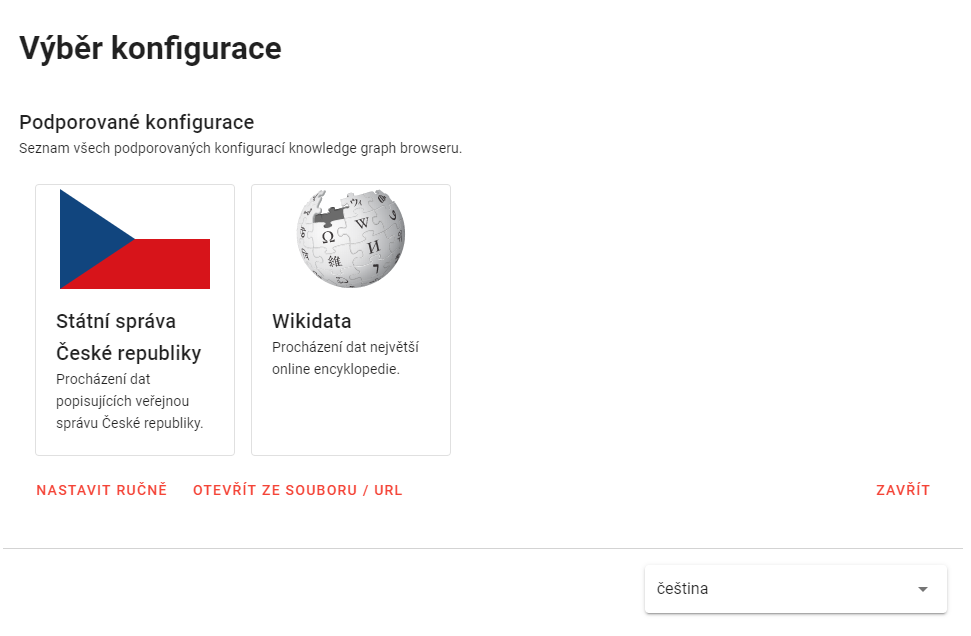
\includegraphics[width=\textwidth]{media/metaconfiguration.png}\\
    \caption{Úvodní obrazovka s výměrem mezi dvěma meta konfiguracemi. Je také možné ručně zadat IRI konfigurací nebo stáhnout graf ze souboru.}
\end{figure}

\newpage

\begin{figure}
    \centering
    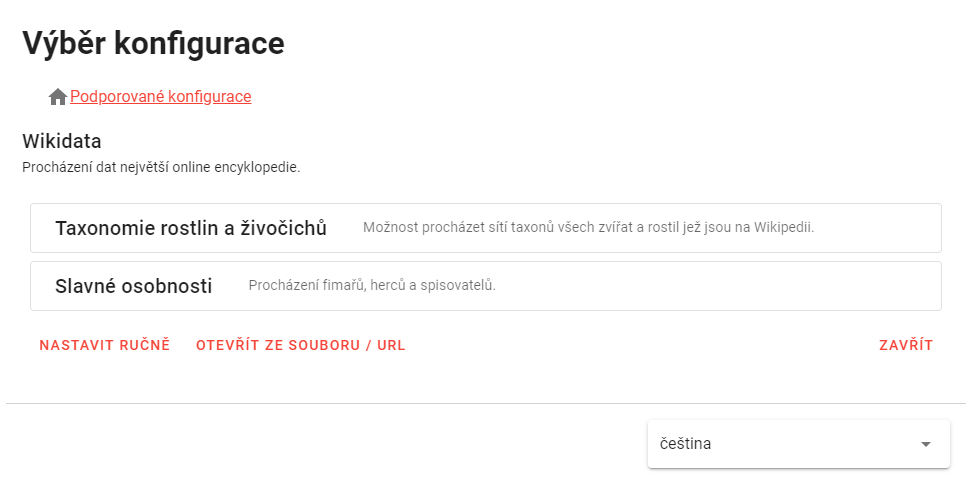
\includegraphics[width=\textwidth]{media/configuration.png}
    \caption{Obrazovka s výběrem konkrétních konfigurací v rámci Wikipedie (Wikidat).}
    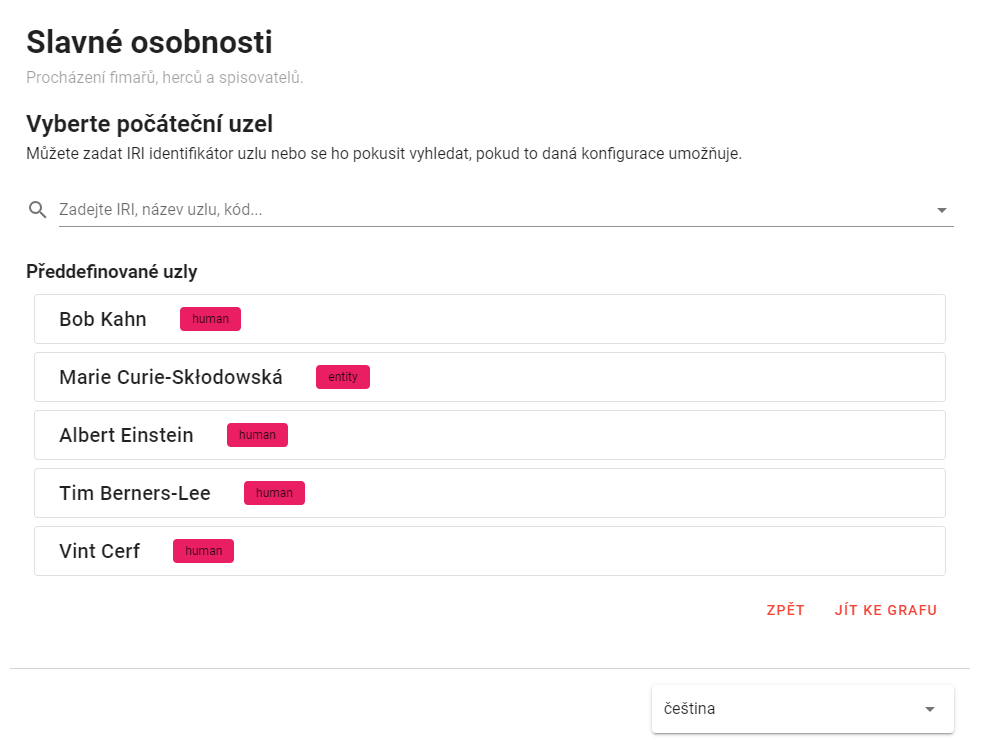
\includegraphics[width=\textwidth]{media/node-selection.png}
    \caption{Obrazovka s výběrem počátečního vrcholu. Ten je možné vybrat z předdefinovaných, nebo je možné použít vyhledávací pole.}
\end{figure}

\newpage

\begin{figure}
    \centering
    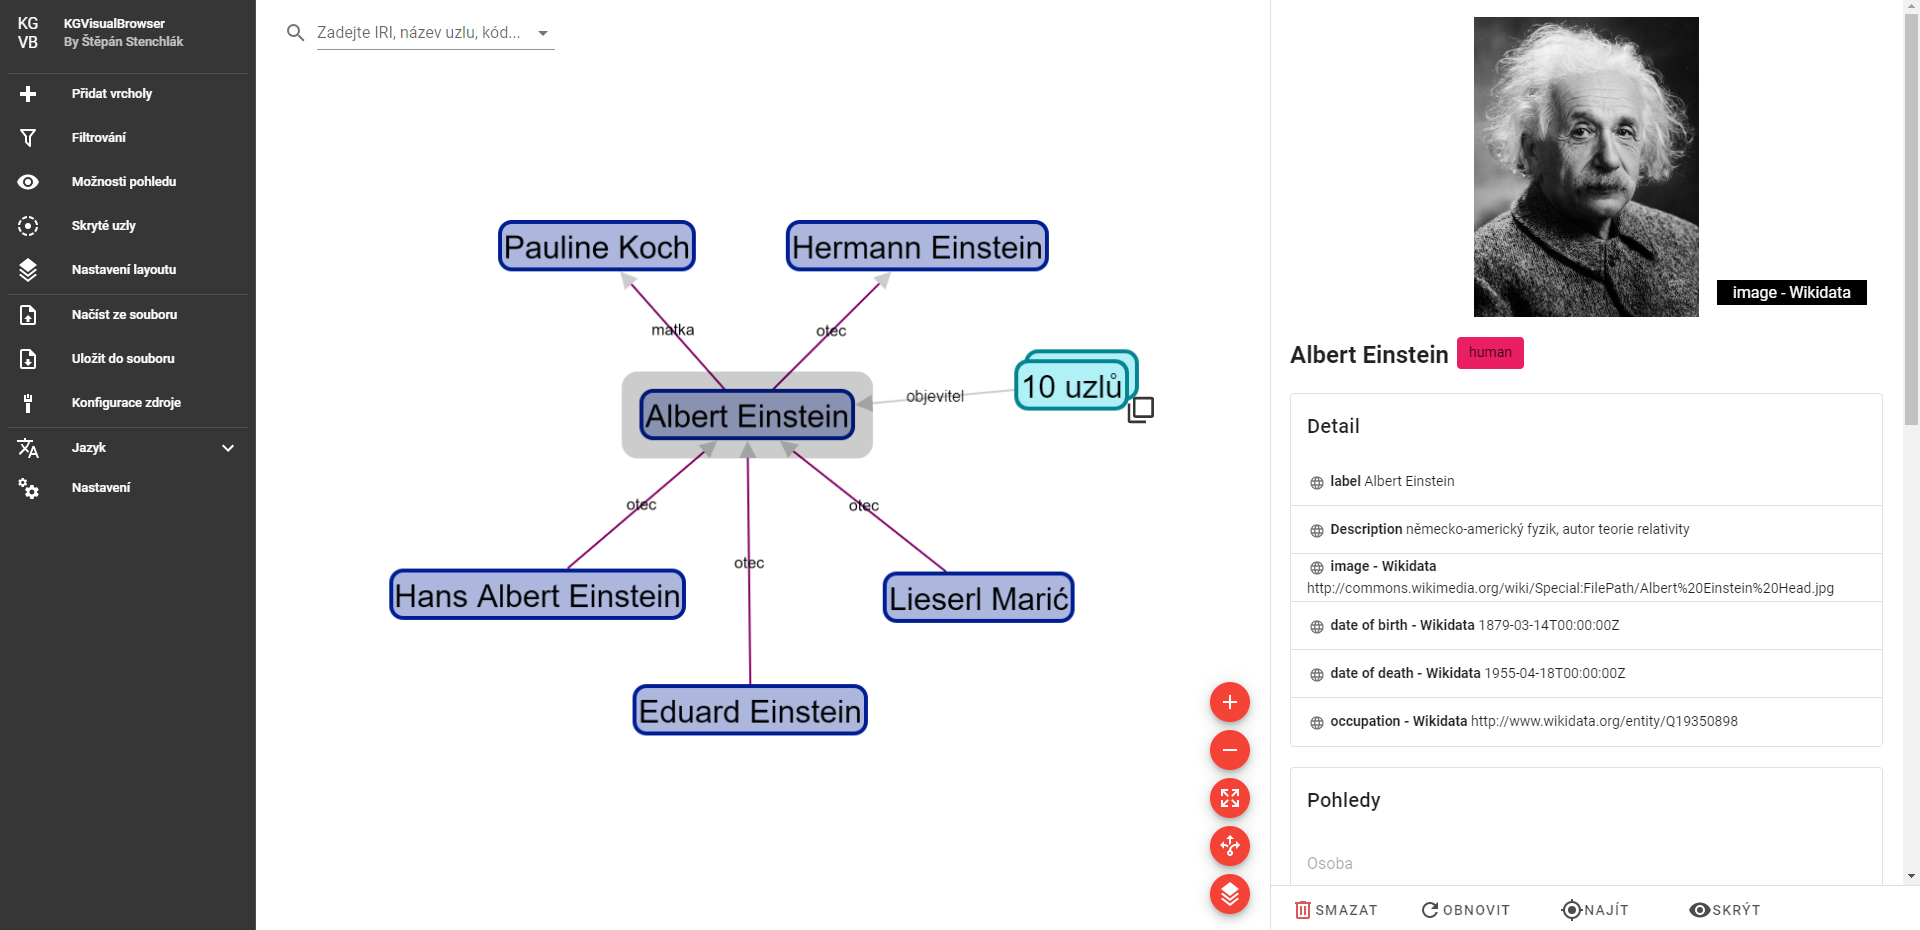
\includegraphics[width=\textwidth]{media/einstein.png}
    \caption{Hlavní okno aplikace s již načteným grafem a vybraným vrcholem. Levý panel je zde rozevřený.}
    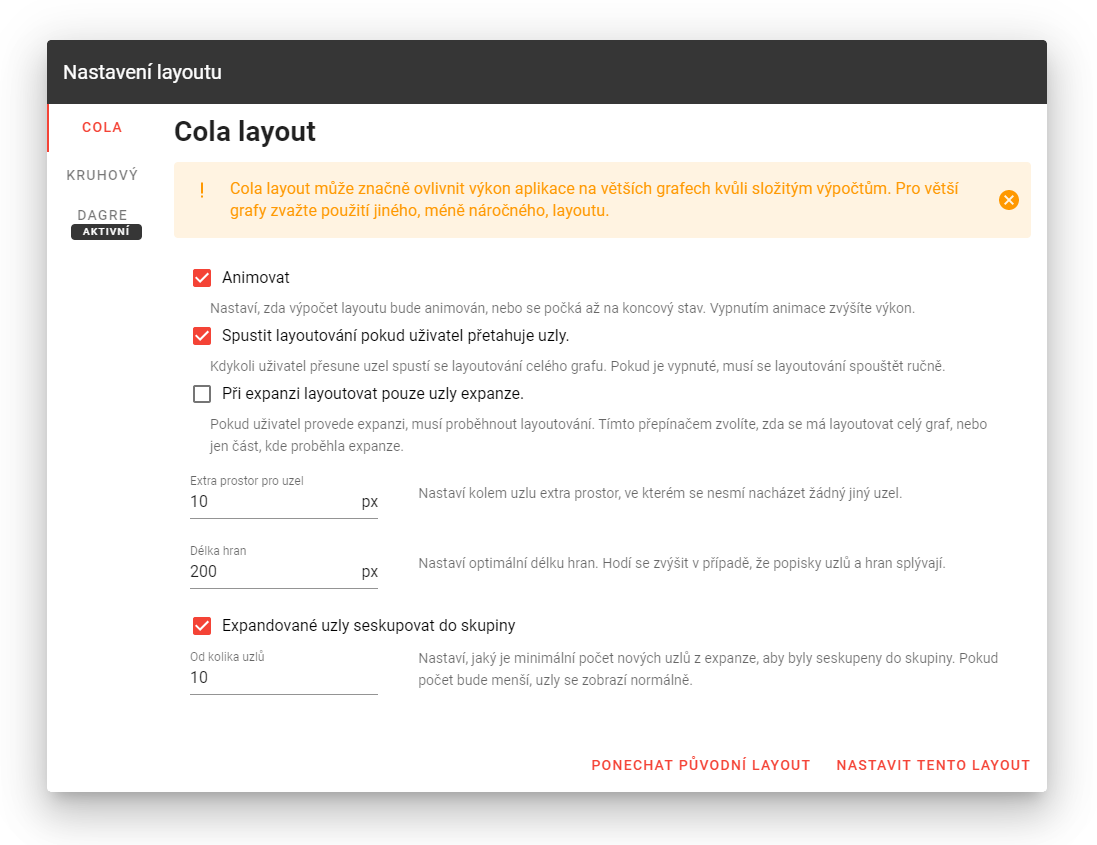
\includegraphics[width=\textwidth]{media/layout.png}
    \caption{Dialog pro výběr a nastavení layoutů.}
\end{figure}